\newpage
\subsection{Hidden Single}
Auch die Technck \textit{Hidden Single} arbeitet wieder mit Kandidatenlisten. Wenn in einer Figur eine Kandidatenliste die einzige ist, in der eine bestimmte Zahl vorkommt, dann kann diese Zahl direkt in die Zelle eingetragen werden. Wenn in dieser Zelle die Zahl nicht stünde, dann gäbe es in der Figur keine Möglichkeit mehr, dass die Zahl auftaucht und damit wäre die Sudoku Regel verletzt, nach der jede Zahl genau einmal enthalten sein muss.

\begin{figure}[h]
\begin{center}
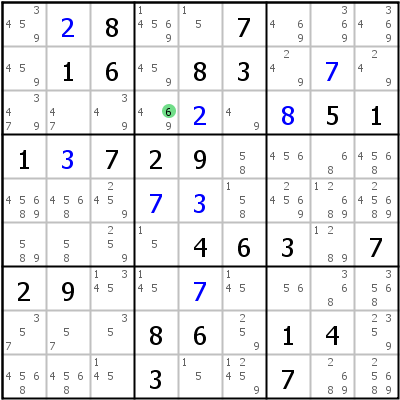
\includegraphics{./img/hidden_single.png}
\caption{Hidden Single}
\end{center}
\end{figure}

In \textbf{Abbildung 3.3} sieht man, dass die Zahl 6 in der Zeile 3 nur in z3s4 vorkommen kann. Daher kann man sie dort eintragen.
